\noindent
\begin{minipage}[t]{0.26\textwidth}
    \vspace*{4.6cm}
    \centering
    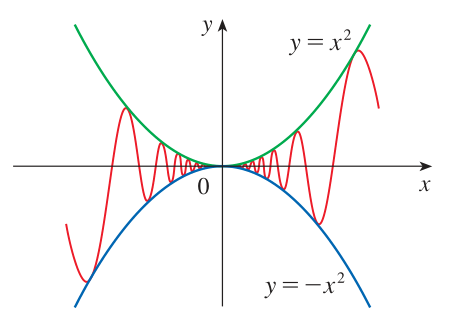
\includegraphics[width=\linewidth]{images/p0137_fig1.png}
    \vspace{2pt}
    \raggedright
    {\small\textbf{\textsf{HÌNH 8}}\quad $y = x^2 \sin(1/x)$}
\end{minipage}%
\hfill
\begin{minipage}[t]{0.71\textwidth}
    \vspace{0pt}
    \noindent\textbf{\textsf{\color{stewartcyan}VÍ DỤ 11}}\quad Chứng minh rằng $\displaystyle\lim_{x \to 0} x^2 \sin \frac{1}{x} = 0$.

    \vspace{0.3em}
    \noindent%
    \begin{tikzpicture}[baseline=-0.6ex]
        \draw[stewartred, fill=stewartred!10, line width=0.8pt, rounded corners=1pt] (0,0) rectangle (0.32,0.32);
        \draw[stewartred, line width=0.8pt] (0,0.32) -- (0.32,0);
        \draw[stewartred, line width=0.6pt] (0.16,0.16) circle (0.09);
    \end{tikzpicture}\hspace{4pt}%
    \textbf{\textsf{\color{stewartcyan}LỜI GIẢI}}\quad Trước tiên lưu ý rằng ta \textbf{không thể} viết lại giới hạn dưới dạng tích của các giới hạn $\lim_{x \to 0} x^2$ và $\lim_{x \to 0} \sin(1/x)$ vì $\lim_{x \to 0} \sin(1/x)$ không tồn tại (xem Ví dụ 2.2.5).

    Ta \textit{có thể} tìm giới hạn bằng cách sử dụng Định lý kẹp. Để áp dụng Định lý kẹp, ta cần tìm một hàm $f$ nhỏ hơn $g(x) = x^2 \sin(1/x)$ và một hàm $h$ lớn hơn $g$ sao cho cả $f(x)$ và $h(x)$ đều tiến tới $0$ khi $x \to 0$. Để làm điều này, ta sử dụng hiểu biết của mình về hàm sin. Vì sin của bất kỳ số nào cũng nằm giữa $-1$ và $1$, ta có thể viết
    
    \vspace{0.2em}
    \noindent
    \begin{tikzpicture}[baseline=(eq.base)]
        \node[draw=stewartred, line width=0.8pt, inner sep=1.8pt, font=\bfseries\footnotesize, text=stewartred] (box) at (0.3,0) {4};
        \node[inner sep=0pt] (eq) at (0.5\linewidth, 0) {$\displaystyle -1 \leqslant \sin \frac{1}{x} \leqslant 1$};
    \end{tikzpicture}

    \vspace{0.2em}
    Bất kỳ bất đẳng thức nào cũng vẫn đúng khi nhân với một số dương. Ta biết rằng $x^2 \geqslant 0$ với mọi $x$ và vì vậy, nhân mỗi vế của các bất đẳng thức trong (4) với $x^2$, ta được
    \[
    -x^2 \leqslant x^2 \sin \frac{1}{x} \leqslant x^2
    \]
    như được minh họa bởi Hình 8. Ta biết rằng
    \[
    \lim_{x \to 0} x^2 = 0 \qquad \text{và} \qquad \lim_{x \to 0} (-x^2) = 0
    \]
    Áp dụng Định lý kẹp với $f(x) = -x^2$, $g(x) = x^2 \sin(1/x)$, và $h(x) = x^2$, ta thu được
    \[
    \lim_{x \to 0} x^2 \sin \frac{1}{x} = 0 \hfill {\color{stewartcyan}\blacksquare}
    \]
\end{minipage}

\vspace{1.2em}

\noindent
\begin{minipage}{\textwidth}
    \parbox[c]{1.3cm}{\fontsize{22}{24}\selectfont\bfseries\color{stewartcyan}\textsf{2.3}}%
    {\color{stewartcyan}\vrule width 1.2pt height 20pt depth 4pt}\hspace{8pt}%
    \parbox[c]{2.6cm}{\fontsize{15}{18}\selectfont\bfseries\textsf{Bài tập}}%
    \hfill
    \parbox[c]{\dimexpr\textwidth - 4.5cm\relax}{%
        \color{stewartcyan!60}%
        \hrule height 0.6pt\vspace{2.5pt}%
        \hrule height 0.6pt\vspace{2.5pt}%
        \hrule height 0.6pt\vspace{2.5pt}%
        \hrule height 0.6pt%
    }
\end{minipage}

\vspace{0.8em}

\noindent
\begin{minipage}[t]{0.485\textwidth}
    \textbf{1.} Cho biết
    \[
    \lim_{x \to 2} f(x) = 4 \qquad \lim_{x \to 2} g(x) = -2 \qquad \lim_{x \to 2} h(x) = 0
    \]
    hãy tìm các giới hạn tồn tại. Nếu giới hạn không tồn tại, hãy giải thích tại sao.

    \vspace{0.4em}
    \noindent
    \begin{tabular}{@{}p{0.48\linewidth}@{\hspace{0.04\linewidth}}p{0.48\linewidth}@{}}
        \textbf{(a)} $\displaystyle \lim_{x \to 2} [f(x) + 5g(x)]$ & \textbf{(b)} $\displaystyle \lim_{x \to 2} [g(x)]^3$ \\[9pt]
        \textbf{(c)} $\displaystyle \lim_{x \to 2} \sqrt{f(x)}$ & \textbf{(d)} $\displaystyle \lim_{x \to 2} \frac{3f(x)}{g(x)}$ \\[14pt]
        \textbf{(e)} $\displaystyle \lim_{x \to 2} \frac{g(x)}{h(x)}$ & \textbf{(f)} $\displaystyle \lim_{x \to 2} \frac{g(x)h(x)}{f(x)}$
    \end{tabular}

    \vspace{1.2em}
    \textbf{2.} Đồ thị của $f$ và $g$ được cho ở hình bên. Hãy sử dụng chúng để tính từng giới hạn, nếu tồn tại. Nếu giới hạn không tồn tại, hãy giải thích tại sao.

    \vspace{0.4em}
    \noindent
    \begin{tabular}{@{}p{0.48\linewidth}@{\hspace{0.04\linewidth}}p{0.48\linewidth}@{}}
        \textbf{(a)} $\displaystyle \lim_{x \to 2} [f(x) + g(x)]$ & \textbf{(b)} $\displaystyle \lim_{x \to 0} [f(x) - g(x)]$ \\[9pt]
        \textbf{(c)} $\displaystyle \lim_{x \to -1} [f(x)g(x)]$ & \textbf{(d)} $\displaystyle \lim_{x \to 3} \frac{f(x)}{g(x)}$
    \end{tabular}
\end{minipage}%
\hfill
\begin{minipage}[t]{0.485\textwidth}
    \noindent
    \begin{tabular}{@{}p{0.48\linewidth}@{\hspace{0.04\linewidth}}p{0.48\linewidth}@{}}
        \textbf{(e)} $\displaystyle \lim_{x \to 2} [x^2 f(x)]$ & \textbf{(f)} $\displaystyle f(-1) + \lim_{x \to -1} g(x)$
    \end{tabular}

    \vspace{0.4em}
    \centering
    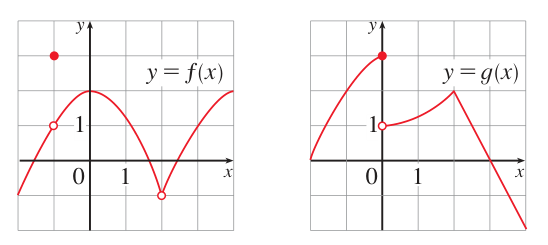
\includegraphics[width=0.92\linewidth]{images/p0137_fig2.png}

    \vspace{0.8em}
    \raggedright
    \noindent\textbf{\textsf{\color{stewartcyan}3--9}}\quad \textbf{Tính giới hạn và giải thích từng bước bằng cách chỉ ra (các) quy tắc giới hạn thích hợp.}

    \vspace{0.5em}
    \noindent
    \begin{tabular}{@{}p{0.50\linewidth}@{\hspace{0.02\linewidth}}p{0.48\linewidth}@{}}
        \textbf{3.} $\displaystyle \lim_{x \to 5} (4x^2 - 5x)$ & \textbf{4.} $\displaystyle \lim_{x \to -3} (2x^3 + 6x^2 - 9)$ \\[12pt]
        \textbf{5.} $\displaystyle \lim_{v \to 2} (v^2 + 2v)(2v^3 - 5)$ & \textbf{6.} $\displaystyle \lim_{t \to 7} \frac{3t^2 + 1}{t^2 - 5t + 2}$ \\[16pt]
        \textbf{7.} $\displaystyle \lim_{u \to -2} \sqrt{9 - u^3 + 2u^2}$ & \textbf{8.} $\displaystyle \lim_{x \to 3} \sqrt[3]{x + 5}\,(2x^2 - 3x)$ \\[16pt]
        \multicolumn{2}{@{}l@{}}{\textbf{9.} $\displaystyle \lim_{t \to -1} \left( \frac{2t^5 - t^4}{5t^2 + 4} \right)^{\!3}$}
    \end{tabular}
\end{minipage}

\vfill
\noindent{\color{stewartcyan}\rule{\linewidth}{0.8pt}}
\vspace{2pt}
\begin{center}
    \fontsize{6.5}{8}\selectfont\color{stewartdarkgray}
    Copyright 2021 Cengage Learning. All Rights Reserved. May not be copied, scanned, or duplicated, in whole or in part. WCN 02-200-203\\ 
    Copyright 2021 Cengage Learning. All Rights Reserved. May not be copied, scanned, or duplicated, in whole or in part. Due to electronic rights, some third party content may be suppressed from the eBook and/or eChapter(s).\\ 
    Editorial review has deemed that any suppressed content does not materially affect the overall learning experience. Cengage Learning reserves the right to remove additional content at any time if subsequent rights restrictions require it.
\end{center}
